\section{Results}
\label{sec:results}

\subsection{Gaussian Splatting}
\paragraph{Hyperparameter tuning.} To accomplish the first goal of this work, producing a dataset of Gaussians accurately representing CIFAR-10 images, we conducted a thorough hyperparameter optimization using the \texttt{gsplat} library. 

As expected, the number of Gaussian primitives used was the most influencing factors on reconstruction quality. We tested using 256, 1024 and 4096 Gaussians, and found 1024 to be a good compromise between reconstruction quality and training efficiency. More interestingly, the opacity regularization factor had a particularly large impact on the optimization result. The initial scale of the Splats also played an important role.  More details about the hyperparameter tuning process can be found in Fig. \ref{}.

\paragraph{Training and dataset generation.}
After finding the optimal hyperparameters for reconstructing the CIFAR-10 images with a high fidelity through Gaussian Splats, we created a dataset reconstructing CIFAR-10 in its entirety using Gaussian Splats. 
L
In addition to the hyperparameters mentioned above, we found out that among the three initialization strategies — random, grid-based and KNN-based — the grid and KNN strategies clearly yielded better reconstructions. For this reason, we decided to generate two datasets of trained splats for the $60,000$ CIFAR-10 images corresponding to these different initialization strategies.

The rasterized images corresponding to the trained Splats resemble the original images accurately for both the grid- and KNN-based initializations, as Fig. \ref{} depicts. While the KNN-based Splats achieved lower losses during training, the grid-based images are visually closer to the original images in general, as can be noticed in the images corresponding to the automobile, deer, truck and ship classes. In some instances, the KNN-based Splats achieved a higher accuracy on local details, such as for the frog's eye or the cat's rings. A further observation is that both initialization strategies struggled with white areas and very bright areas of the images. This is particularly evident for the cat class and smaller areas of other images,
such as the back of the automobile image. This problem is slightly more prominent for the KNN-based initialization. 

Both generated Gaussian Splat datasets were implemented as \texttt{PyTorch} datasets using a 4 : 1 : 1 split for training, validation, and test sets. The full datasets have a size of approximately 5 GB.

\begin{figure*}
    \centering
    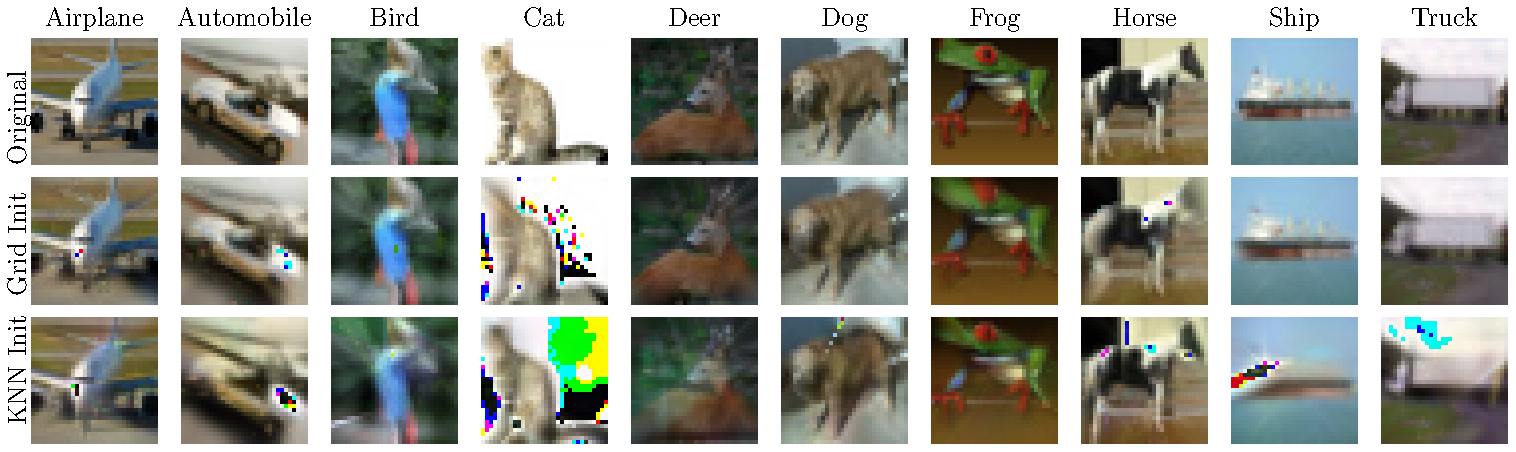
\includegraphics[width=1\linewidth]{fig/splat_reconstruction_comparison.pdf}
    \caption{\textbf{Gaussian Splat Reconstruction of the CIFAR-10 Classes.} Example reconstructions for one of each CIFAR-10 classes. The top row shows the original image, while the middle and lower rows show the Gaussian Splat reconstructions using the grid- and KNN-initializations respectively.}
    \label{fig:splat-reconstructions}
\end{figure*}

\subsection{Auto-encoding of 2D Splats}
\paragraph{Model comparison.} TODO: write on the performance (quality of the reconstruction for each model)
TODO: loss plot here, emphasize that we did hyperparameter tuning for all models on the plot  -> maybe mention the hyperparams used or use a small table.
TODO: write on the compute performance + limitation of model 2 to using batchsize 1

\paragraph{Reconstructing the original images.}
TODO: put in the image of the generated outputs of one model of each class, maybe cherrypick